%!TEX root = ../Chapter4.tex

\section{Experiments}\label{sec:lgc.experiments}

In this section, we provide technical details of our experiments. We also share a few insights over different aspects of implementations of different pure exploration linear bandits algorithms. In particular, we propose a new Frank-Wolfe-typed heuristic to solve generic $\cA\cB$-design.

Besides our algorithms, we implement the following algorithms, all using the same stopping rule (more discussion given in Appendix~\ref{app:lgc.stopping}): uniform sampling, the greedy version of \XYS (including $\gopt$-allocation and $\xyopt$-allocation), \XYA, and the greedy version of \LGapE. We skip \GLUCB/\GLGapE since they are more or less equivalent to \LGapE in the scope of this paper.

\subsection{Implementation details}\label{sec:lgc.experiments.implem}

\paragraph{More details for algorithm implementations.} We give more clarifications on each individual algorithm implemented.

\begin{itemize}
	\item For our algorithms \LG and \LGC, we implemented the version with the boundedness assumption.
	\item For \LGapE We implemented the greedy version, that is, pull the arm 
	\[
	    \argmin_{a\in\cA} \normm{a_{i_t}-a_{j_t}}_{(V_{N_t}+aa^\top)^{-1}}^2
	\]
	with $i_t = i^\star(\hat\theta_t)$ and $j_t = \argmax_{j\neq i_t}\langle\hat\theta_t,a_{j}-a^\star(\hat\theta_t)\rangle + \normm{a^\star(\hat\theta_t) - a_{j_t}}_{V_{N_t}^{-1}} \sqrt{2\beta(t,\delta)}$. Note that this version does not have a theoretical guarantee in the general case. However, as we stated in Section~\ref{sec:lgc.related_work}, the \GLUCB proposed by~\citet{zaki2019maxoverlap} is equivalent to this greedy version of \LGapE, and they provided an analysis for the 2-arm and 3-arm case. \LGapE is designed for $\epsilon$-best-arm identification, we set $\epsilon=0$ in our experiments to make sure that it outputs the optimal one.
	\item For \XYS, we implemented the greedy incremental version for both $\gopt$-allocation and $\xyopt$-allocation, that allows us to avoid the optimal design-computing step. To implement the non-greedy version, readers are invited to look at next Section~\ref{sec:lgc.experiments.complexity} where we discuss in detail the computation of $\cA\cB$-optimal design.
	\item For \XYA, it requires a hyper-parameter that characterizes the length of each phase. We set that hyper-parameter to $0.1$ as done by~\citet{soare2014linear}.
\end{itemize}

\paragraph{Technical details.} All the algorithms and experiments are implemented in \lstinline{Julia 1.3.1}, and plots are generated using the \lstinline{StatsPlots.jl} package. Other external dependencies are: \lstinline{JLD2.jl, Distributed.jl, IterTools.jl, CPUTime.jl, LaTeXStrings.jl}.

\paragraph{For reproducibility.} To rerun our code, your need to have Julia installed, then unzip \lstinline{code.zip} and do the following in your terminal.

\begin{lstlisting}
  $ cd PATH/TO/THE/FOLDER/code/linear
  $ julia
  julia> include("experiment_bai1.jl") # reproduce Fig.1
  julia> include("viz_bai1.jl") # visualization
  julia> include("experiment_bai2.jl") # reproduce Fig.2
  julia> include("viz_bai2.jl") # visualization
\end{lstlisting}

%\subsubsection{Arm generation.} In Section~\ref{sec:experiments}, we need to generate arms uniformlly from a unit sphere of arbitrary dimension. This can be done using Algorithm~\ref{alg:generation}, it can be trivially extended to higher dimension.
%
%\begin{algorithm}[ht]
%   \caption{Generating arms from the 2D unit sphere (Box-Mueller)}
%   \label{alg:generation}
%\begin{algorithmic}
%        \State $u \sim \cN(0,1)$
%        \State $v \sim \cN(0,1)$
%        \State $(x, y) = (u, v)/\normm{(x, y)}_2$
%        \RETURN $x, y$
%\end{algorithmic}
%\end{algorithm}

\subsection{Computation of different complexities}\label{sec:lgc.experiments.complexity}

As mentioned in Section~\ref{sec:lgc.lower_bound}, computing the solution to a specified optimization problem is required in many existing linear BAI algorithms. We survey some methods that can potentially be useful to handle that issue.

We recall that the three notions of complexity $\gopt, \xyopt, \cA\cBstar(\theta)$ can be written in a unified form,
\begin{align}\label{eq:complexity_general}
    \cA\cB = \min_{w\in\Sigma_A} \max_{b\in\cB}\normm{b}_{V_w^{-1}}^2,
\end{align}
where $\cB$ is the transductive set, i.e. a finite set of elements in $\R^d$. Transductive sets corresponding to different complexity types mentioned in this paper can be found in Table~\ref{tab:transductive_sets}.

\begin{table}[ht]
    \centering
	\begin{tabular}{@{}lll@{}}
		\toprule
		\thead{Allocation type} & \thead{Arm set} & \thead{Transductive set} \\ \midrule
		(1) $\gopt$-allocation & $\cA$ & $\cA$\\
		(2) $\xyopt$-allocation & $\cA$ & $\cB_{\texttt{dir}} = \{a-a':\ (a,a')\in\cA\times\cA\}$ \\
		(3) $\cA\cBstar(\theta)$-allocation & $\cA$ & $\cB^\star(\theta) = \left\{ (\astar(\theta)- a)/\left|\big\langle \theta, \astar(\theta)-a\big\rangle\right|: a\in\cA/\big\{\astar(\theta)\big\}  \right\}$ \\
		\bottomrule
	\end{tabular}
	\caption{Some examples of different transductive sets.}
	\label{tab:transductive_sets}
\end{table}

\paragraph{Frank-Wolfe.} We can use a Frank-Wolfe heuristic to compute the optimizer of~\eqref{eq:complexity_general} shown in Algorithm~\ref{alg:fw_aa}. This heuristic is used for example by~\citet{fiez2019transductive}. Note that this heuristic has been proved to have a linear convergence guarantee when $\cB = \cA$~\citep{ahipasaoglu2008fw}. It is not clear, however, that the same guarantee holds for other transductive sets.

A simple sanity check to test whether a solver works smoothly is  to solve $\cA\cBstar(\theta)$ for classical multi-armed bandits (i.e. when $\cA= \{e_1,e_2,\ldots,e_d\}$), for which a solver with guarantee exists (see \citealt{garivier2018explore}). In particular we found instances where Algorithm~\ref{alg:fw_aa} does not converge toward the optimal weights, for example: $\cA= \{e_1,e_2,e_3\}, \theta = (0.9, 0.5, 0.5)$.

% \begin{algorithm}[ht]
%    \caption{Frank-Wolfe heuristic for computing $\gopt$-design}
%    \label{alg:fw_aa}
% \begin{algorithmic}
%    \State {\bfseries Input:} arm set $\cA\subset\R^d$, transductive set $\cB\subset\R^d$, maximum iterations $n$
%    \State  {\bfseries Initialize:} $w \leftarrow{} (1/A, 1/A, \ldots, 1/A), V \leftarrow{} I_d, t \leftarrow{} 0$
%    \While{$t<n$}
%         \State $i_{t}\in\argmin_{i\in\{1,\ldots,A\}}\max_{b\in\cB}\normm{b}^2_{(V+a_i a_i^\top)^{-1}}$
%         \State $V \leftarrow{} V + a_{i_{t}}a_{i_{t}}^\top$
%         \State $w \leftarrow{} \frac{t}{t+1}w+\frac{1}{t+1}e_{i_{t}}$
%         \State $t \leftarrow{} t+1$
%    \EndWhile
%    \RETURN $w$
% \end{algorithmic}
% \end{algorithm}


\begin{algorithm}[ht]
\centering
\caption{Frank-Wolfe heuristic for computing $\gopt$-design}
\label{alg:fw_aa}
\begin{algorithmic}
   \State {\bfseries Input:} arm set $\cA\subset\R^d$, transductive set $\cB\subset\R^d$, maximum iterations $n$
   \State  {\bfseries Initialize:} $w \leftarrow{} (1, 1, \ldots, 1)\in\R^A, V \leftarrow{} I_d, t \leftarrow{} 0$
   \While{$t<n$}
        \State $\ta\in\argmin_{a\in\cA}\max_{b\in\cB}\langle a,b\rangle_{V^{-1}}^2$%\normm{b}^2_{(V+a_i a_i^\top)^{-1}}$
        \State $V \leftarrow{} V + \ta \ta^\top$
        \State $w \leftarrow{} \frac{t}{t+1}w+\frac{1}{t+1}e_{\ta}$
        \State $t \leftarrow{} t+1$
   \EndWhile
   \State {\bfseries Return} $w$
\end{algorithmic}
\end{algorithm}

We propose a variant of the previous heuristic that takes into account a count for each element in the transductive set $\cB$. The pseudo-code of our method is displayed in Algorithm~\ref{alg:fw_ab}. $N\in\NN^{|\cB|}$ denotes the vector of counts for all $b\in\cB$. Sanity check on various MAB instances shows the correctness of our heuristic, its convergence guarantee remains for the future work.

% \begin{algorithm}[ht]
%    \caption{Saddle Frank-Wolfe heuristic for computing generic $\cA\cB$-design}
%    \label{alg:fw_ab}
% \begin{algorithmic}
%    \State {\bfseries Input:} arm set $\cA\subset\R^d$, transductive set $\cB\subset\R^d$, maximum iterations $n$
%    \State  {\bfseries Initialize:} $w \leftarrow{} (1/A, 1/A, \ldots, 1/A), N \leftarrow{} (1, 1, \ldots, 1), V \leftarrow{} I_d, t \leftarrow{} 0$
%    \While{$t<n$}
%         \State $i_{t}\in\argmin_{i\in\{1,\ldots,A\}}\sum_{j=1}^B(-2N[j]\langle a_i,V b_j\rangle^2)$
%         \State $j_{t}\in\argmax_{j\in\{1,\ldots,B\}}\normm{b_{j}}^2_{V^{-1}}$
%         \State $V \leftarrow{} V + a_{i_{t}}a_{i_{t}}^\top$
%         \State $N[j_t] \leftarrow{} N[j_t] + 1$
%         \State $w \leftarrow{} \frac{t}{t+1}w+\frac{1}{t+1}e_{i_{t}}$
%         \State $t \leftarrow{} t+1$
%    \EndWhile
%    \RETURN $w$
% \end{algorithmic}
% \end{algorithm}

\begin{algorithm}[ht]
\centering
\caption{Saddle Frank-Wolfe heuristic for computing generic $\cA\cB$-design}
\label{alg:fw_ab}
\begin{algorithmic}
   \State {\bfseries Input:} arm set $\cA\subset\R^d$, transductive set $\cB\subset\R^d$, maximum iterations $n$
   \State  {\bfseries Initialize:} $w \leftarrow{} (1, 1, \ldots, 1)\in\R^A, \tV \leftarrow{} I_d, V \leftarrow{} I_d, t \leftarrow{} 0$
   \While{$t<n$}
        \State $\ta\in\argmax_{a\in\cA}  \norm{a}_{V^{-1} \tV V^{-1} }^2$
        \State $\tb\in\argmax_{b\in\cB}\normm{b}^2_{V^{-1}}$
        \State $V \leftarrow{} V + \ta\ta^\top$
		\State $\tV \leftarrow{} \tV + \tb\tb^\top$
        \State $w \leftarrow{} \frac{t}{t+1}w+\frac{1}{t+1}e_{\ta}$
        \State $t \leftarrow{} t+1$
   \EndWhile
   \State {\bfseries Return} $w$
\end{algorithmic}
\end{algorithm}

\paragraph{Entropic mirror descent.}
An entropic mirror descent alternative is used by~\citet{tao2018alba} to compute $\gopt$. The entropic mirror descent approach requires the knowldge of the Lipschitz constant of $\log\det V_w$. Unfortunately, that Lipschitzness property does not seem to hold. \citet{lu2018convex} propose a solution to overcome the Lipschitz issue, but only for $\gopt$-design. Whether it still works for general $\cA\cB$-design remains an open question.

%\begin{algorithm}[ht]
%   \caption{Entropic mirror descent heuristic for computing $\gopt$-design}
%   \label{alg:algoMD}
%\begin{algorithmic}
%   \State {\bfseries Input:} arm set $\cA\subset\R^d$, transductive set $\cB\subset\R^d$, tolerance constant $\epsilon$, Lipschitz constant $L$
%   \State  {\bfseries Initialize:} $w \leftarrow{} (1/A, 1/A, \ldots, 1/A), t \leftarrow{} 1$
%   \While{$|\max_{a\in\cA}a^\top V_w^{-1} a - d| \geq \epsilon$}
%        \State $\gamma \leftarrow{} \frac{2\sqrt{A}}{L} \frac{1}{\sqrt{t}}$
%        \State Compute gradient $\nabla^i \leftarrow{} \Tr(V_w^{-1}a_ia_i^\top)$
%        \State $w^{a_i} \leftarrow{} \frac{w^{a_i}\exp(\gamma \nabla^i)}{\sum_{i=1}^A w^{a_i}\exp(\gamma \nabla^i)}$
%        \State $t \leftarrow{} t+1$
%   \EndWhile
%   \RETURN $w$
%\end{algorithmic}
%\end{algorithm}

\subsection{Implementation tricks}\label{sec:lgc.experiments.tricks}

\paragraph{Rank-1 matrix inversion and posterior update.}
Matrix inversion is a costly step that should be avoided at best. For linear bandits, in particular, we need to inverse the (regularized) design matrix $\bB^{\lambda}_n$, which is renewed with a rank-1 update at each time step. Applying Sherman-Morrison formula allows us thus to only update its inverse incrementally, that releases a huge burden of computation.

Indeed, beginning with $\bB^{\lambda}_0 \eqdef \lambda\1_d$, we have
\[
    \forall t\geq 0, \quad \bB^{\lambda}_{t+1} = \bB^{\lambda}_t + \hat{\bx}_{t+1}\hat{\bx}_{t+1}\transpose,
\]
thus using Sherman-Morrison formula we have
\[
    \forall t\geq 0, \quad (\bB^{\lambda}_{t+1})^{-1} = (\bB^{\lambda}_t)^{-1} - \frac{(\bB^{\lambda}_t)^{-1}\hat{\bx}_{t+1}\hat{\bx}_{t+1}\transpose(\bB^{\lambda}_t)^{-1}}{1+\normm{\hat{\bx}_{t+1}}_{(\bB^{\lambda}_t)^{-1}}^2}.
\]

The posterior mean vector and covariance matrix can then be easily expressed in terms of $(\bB^{\lambda}_t)^{-1}$. Let $\bz_t \eqdef \sum_{s=1}^t y_s\hat{\bx}_s$, we obtain
\[
    \hat{\btheta}_n^{\lambda} = (\bB^{\lambda}_t)^{-1}\bz_t \quad \text{and} \quad \hat{\bSigma}_n = \sigma^2 (\bB^{\lambda}_t)^{-1}.
\]

\paragraph{Rank-1 multivariate normal distribution sampling}
A random Gaussian vector 
\[
    \bX = (X_1, X_2, \ldots, X_d)\transpose
\] 
of mean vector $\bar{\bmu}$ and covariance matrix $\bSigma$ can be formally defined as following,
\[
    \bX \sim \cN(\bar{\bmu}, \bSigma) \iff \exists \bar{\bmu}\in\mathbb{R}^d,\bA\in\mathbb{R}^{d\times d'} \ \text{s.t.} \ \bX = \bA \mathbf{Z} + \bar{\bmu},
\]
for $Z_i \sim\ \mathcal{N}(0, 1)$ i.i.d. with $i\in\{1,\ldots,d'\}$, and here $\bSigma = \bA\bA\transpose$.

To draw a sample from a multivariate normal distribution, according to the previous definition, one can first find any real matrix $\bA$ such that $\bA\bA\transpose = \bSigma$. Then draw a vector $\bZ$ whose components independently follow standard normal distribution. Finally $\bX = \bA \mathbf{Z} + \bar{\bmu}$ forms a valid sample. The main issue is thus how to find an appropriate matrix $\bA$.

In this chapter, we need to sample from $\cN(\hat{\btheta}^\lambda_n,\hat{\bSigma}_n)$ for \LTCC{} for example, where the covariance matrix $\hat{\bSigma}_n$ is a positive-definite matrix. A usual way is to apply the Cholesky decomposition, which is computationally inefficient if it were to be applied at each time step. Fortunately, we can apply rank-1 Cholesky decomposition in our case.  

%We, however, notice that $\bA = (\hat{\bSigma}_n)^{1/2}=\sigma(\bB^{\lambda}_n)^{-1/2}$ is also a valid candidate, and is thus can be also updated iteratively using a similar formula to the Sherman-Morrison formula.

%More precisely, we have
%\begin{align*}
%    \forall t\geq 0, \quad (\bB^{\lambda}_{t+1})^{-\frac{1}{2}} = (\bB^{\lambda}_t)^{-\frac{1}{2}} - \ddfrac{\left(1-\sqrt{1-\frac{\normm{\hat{\bx}_{t+1}}_{(\bB^{\lambda}_t)^{-1}}^2}{1+\normm{\hat{\bx}_{t+1}}_{(\bB^{\lambda}_t)^{-1}}^2}}\right)}{\normm{\hat{\bx}_{t+1}}_{(\bB^{\lambda}_t)^{-1}}^2} (\bB^{\lambda}_t)^{-\frac{1}{2}}\hat{\bx}_{t+1}\hat{\bx}_{t+1}\transpose(\bB^{\lambda}_t)^{-\frac{1}{2}}.
%\end{align*}

\subsection{Experimental setting}\label{sec:lgc.experiments.setting}

\paragraph{The usual hard instance.}
Usual sampling rules for classical BAI may not work for the linear case. This can be understood on a well-studied instance already discussed by~\citet{soare2014linear,xu2018linear}, which encapsulates the difficulty of BAI in a linear bandit, and thus is the first instance on which we test our algorithms. In this instance, arms are the canonical basis  $a_1 = e_1, a_2 = e_2, a_d = e_d$, plus an additional disturbing arm $a_{d+1} = (\cos(\alpha), \sin(\alpha), 0, \ldots, 0)^\top$, and a true regression parameter $\theta$ equal to $e_1$. In this problem, the best arm is always $a_1$, but when the angle $\alpha$ is small, the disturbing arm $a_{d+1}$ is hard to discriminate from $a_1$. As already argued by~\citet{soare2014linear}, an efficient sampling rule for this problem instance would rather pull $a_2$ in order to reduce the uncertainty in the direction $a_1-a_{d+1}$. Naive adaptation of classical BAI algorithms cannot deal with that situation naturally. We further use a simple set of experiments to justify that intuition. We run our two algorithms and the one of~\citet{degenne2019game} that we call \texttt{DKM} over the problem instance whence $d=2$, $\delta=0.01$ and $\alpha=0.1$. We show the number of pulls for each arm averaged over 100 replications of experiments in Table~\ref{table:pulls}. We see that, indeed, \texttt{DKM} pulls too much $a_3$, while our algorithms focus mostly on $a_2$.

\begin{table}[t!]\centering
%\def\arraystretch{1.2}
\begin{tabular}{|c|c|c|c|}
 \hline
 & \LG & \LGC & \texttt{DKM} \\
 \hline
 \textbf{$a_1$} & $1912$ & $1959$ & $1943$ \\
 \hline
 \textbf{$a_2$} & $5119$ & $4818$ & $4987$ \\
 \hline
 \textbf{$a_3$} & $104$ & $77$ & $1775$ \\
 \hline
 \textbf{Total} & $7135$ & $\bf{6854}$ & $8705$ \\
 \hline
\end{tabular}
\caption{Average number of pulls of \LG and \LGC (against \texttt{DKM}) for each arm.}
\label{table:pulls}
\end{table}

\subsection{Experimental results}\label{sec:lgc.experiments.results}

\paragraph{Comparison of different complexities.}
We use the previous setting to illustrate various complexities differ in practice. In Table~\ref{table:optimal_weights} we compare the different complexities mentioned in this paper: the characteristic time $\Tstar(\theta)$ and its associated optimal weights $\wstar_{\cA\cBstar(\theta)}$, the $\xyopt$-complexity and its associated optimal design $\wstar_{\xyopt}$, the G-optimal complexity $\gopt$ and its associated optimal design $\wstar_{\cA\cA}$. For each weight vector $w \in\{\wstar_{\cA\cBstar(\theta)},w_{\xyopt}, w_{\gopt}\}$,
 we also provide the lower bound $T_w$ given by Theorem~\ref{th:lb_genral}, i.e.
 \[
 T_w = \max_{a\neq \astar(\theta)} \frac{\big\langle \theta, \astar(\theta)-a\big\rangle^2}{2\normm{\astar(\theta)-a}_{V_w^{-1}}^2} \log(1/\delta).
\]
In particular we notice that targeting the proportions of pulls $w_{\xyopt}, w_{\gopt}$ leads to a much larger lower bound than the one obtained with the optimal weights.
\begin{table}[t!]
\centering
%\def\arraystretch{1.2}
\begin{tabular}{|c|c|c|c|}
 \hline
   & $\wstar_{\cA\cBstar}$ & $\wstar_{\xyopt}$  & $\wstar_{\gopt}$   \\
 \hline
 \textbf{$a_1$} & $0.047599$ & $0.499983$ & $0.499983$ \\
 \hline
 \textbf{$a_2$} & $0.952354$ & $0.499983$ & $0.499983$ \\
 \hline
 \textbf{$a_3$} & $0.000047$ & $0.000033$ & $0.000033$ \\
 \hline
 \textbf{$T_w$} & $369$ & $2882$ & $2882$ \\
 \hline
   & $\Tstar(\theta)$ & $2\xyopt/\DeltaMin^2$ & $8\gopt/\DeltaMin^2$\\
 \hline
  \textbf{Complexity} & $0.124607$ & $32.0469$ & $64.0939$ \\
 \hline
\end{tabular}
\caption{Optimal weights for various complexities with $\DeltaMin= 0.0049958$.}
\label{table:optimal_weights}
\end{table}

\paragraph{Comparison with other algorithms.}
Finally we benchmark our two sampling rules against others from the literature. %Note that the main purpose of this paper is to propose algorithms with asymptotic optimality while being practically usable, but we do not claim to have the best performing ones.
We test over two synthetic problem instances, with the first being the previous counter-example. We set $d=2$, $\alpha=\pi/6$. Fig.~\ref{fig:sample_complexity_1} shows the empirical stopping time of each algorithms averaged over 100 runs, with a confidence level $\delta=0.1, 0.01, 0.0001$ from left to right. Our two algorithms show competitive performance (the two leftmost boxes on each plot), and are only slightly worse than \LGapE.

\begin{figure}[ht]
 \centering
 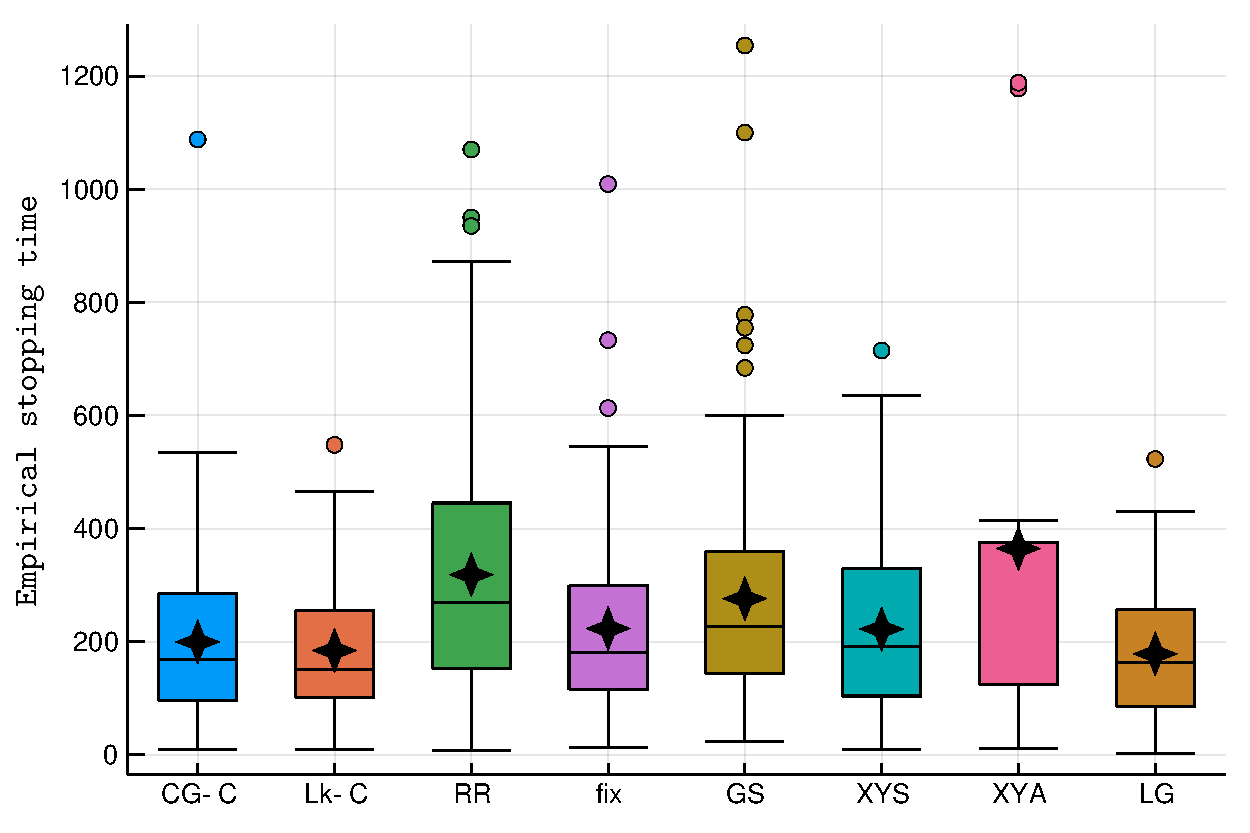
\includegraphics[clip, width= 0.33\textwidth]{Chapter4/img/bai_sin_0-1}
 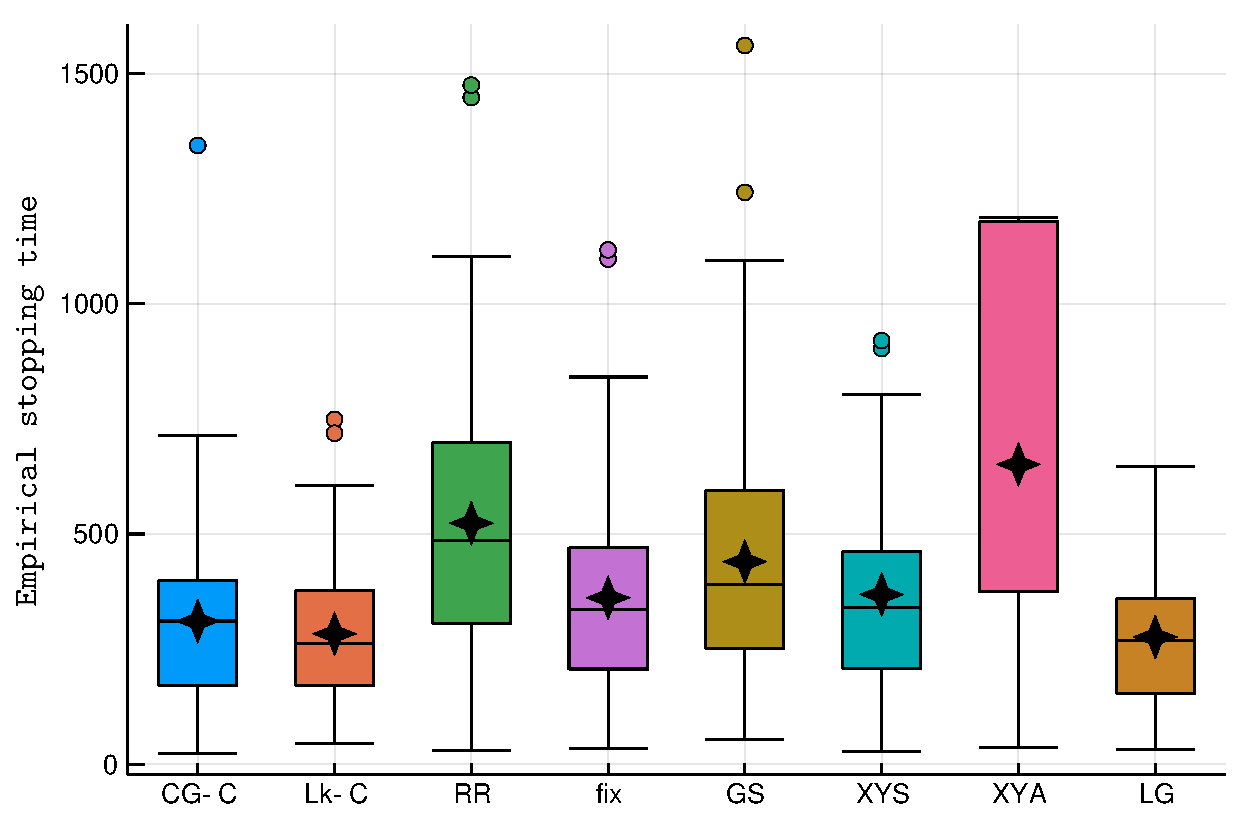
\includegraphics[clip, width= 0.33\textwidth]{Chapter4/img/bai_sin_0-01}
 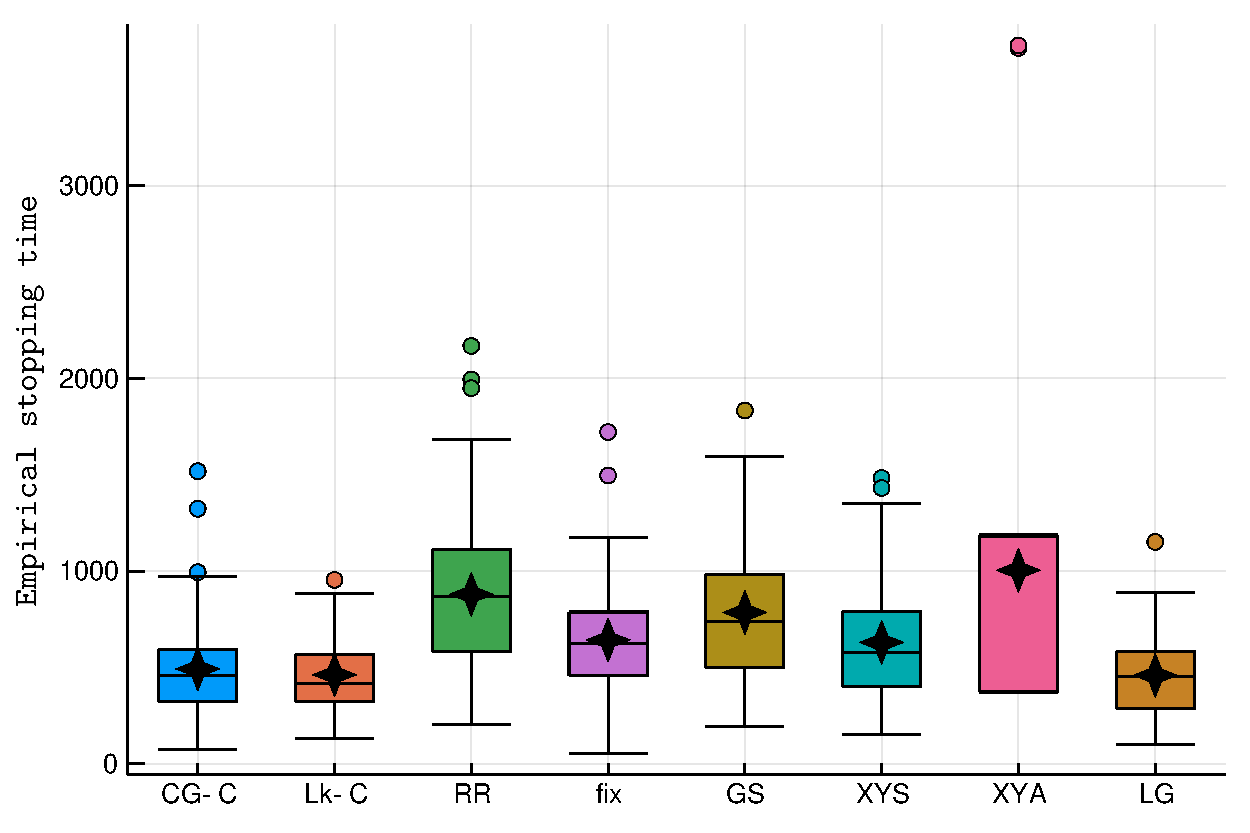
\includegraphics[clip, width= 0.33\textwidth]{Chapter4/img/bai_sin_0-0001}
 \caption{Sample complexity of different linear BAI sampling rules over the usual counter-example with $\delta=0.1, 0.01, 0.0001$ respectively. CG = \LGC,  Lk = \LG, RR = uniform sampling, fix = tracking the fixed weights, GS = \XYS with $\gopt$-allocation, XYS = \XYS with $\xyopt$-allocation, LG = \LGapE. The mean stopping time is represented by a black cross.}
 \label{fig:sample_complexity_1}
\end{figure}

For the second instance, we consider 20 arms randomly generated from the unit sphere $\mathbb{S}^{d-1}\eqdef\{a\in\R^d; \normm{a}_2=1\}$. We choose the two closest arms $a, a'$ and we set $\theta = a + 0.01(a'-a)$ so that a is the best arm. This setting has already been considered by~\citet{tao2018alba}. We report the same box plots over 100 replications as before with increasing dimension in Fig.~\ref{fig:sample_complexity_2}. More precisely, we set $d=6, 8, 10, 12$ respectively, and always keep a same $\delta = 0.01$. Our algorithms consistently show strong performances compared to other algorithms apart from \LGapE. Moreover, we can see that in these random examples, \LGC works better than the non-confexified one, and is even competitive compared to \LGapE.


\begin{figure}[ht]
 \centering
 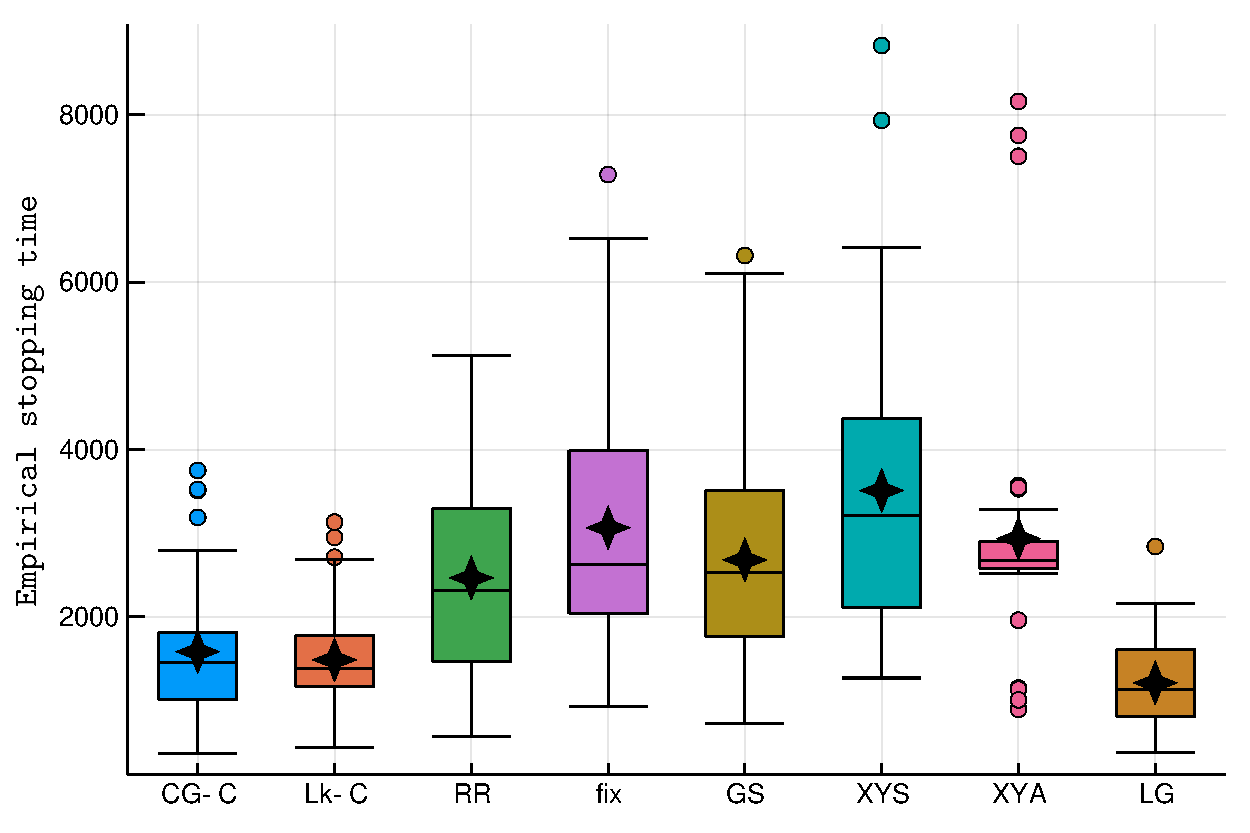
\includegraphics[clip, width= 0.33\textwidth]{Chapter4/img/bai_dim_6}
 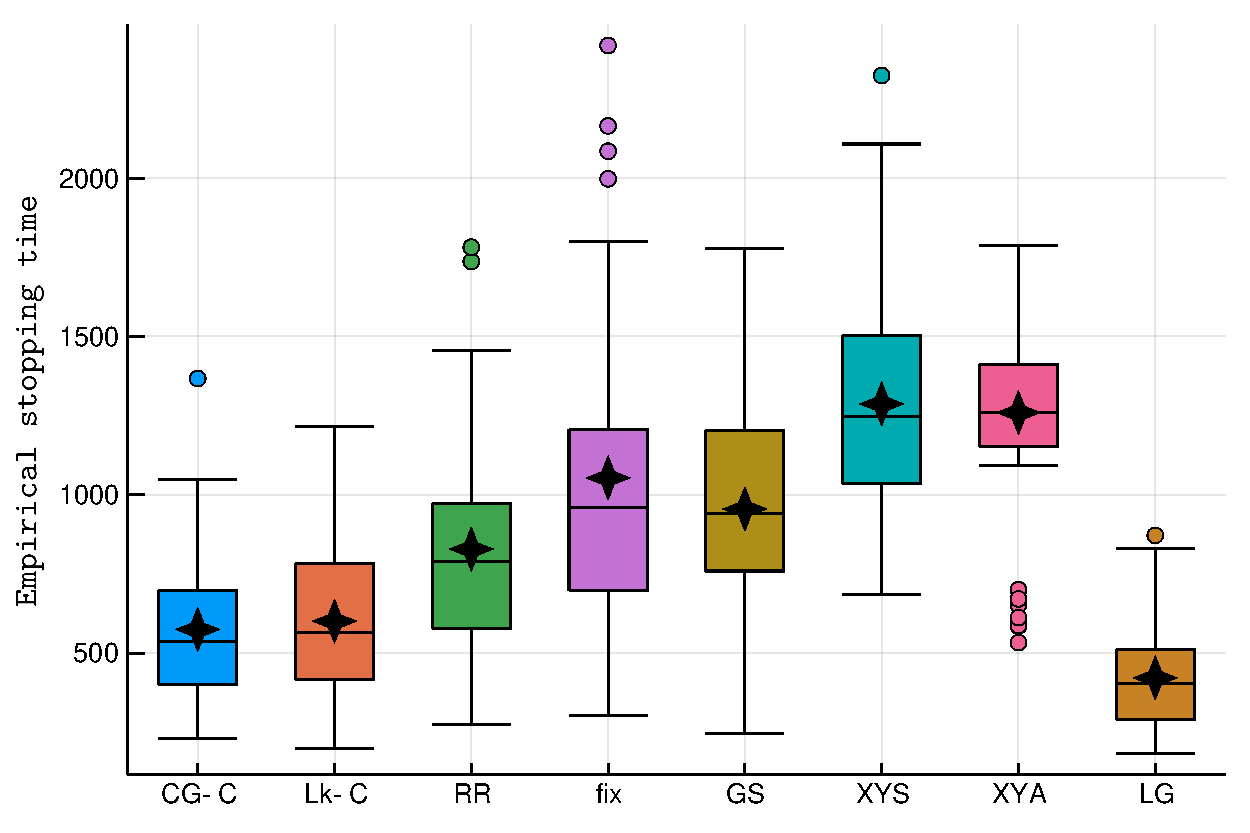
\includegraphics[clip, width= 0.33\textwidth]{Chapter4/img/bai_dim_8}
 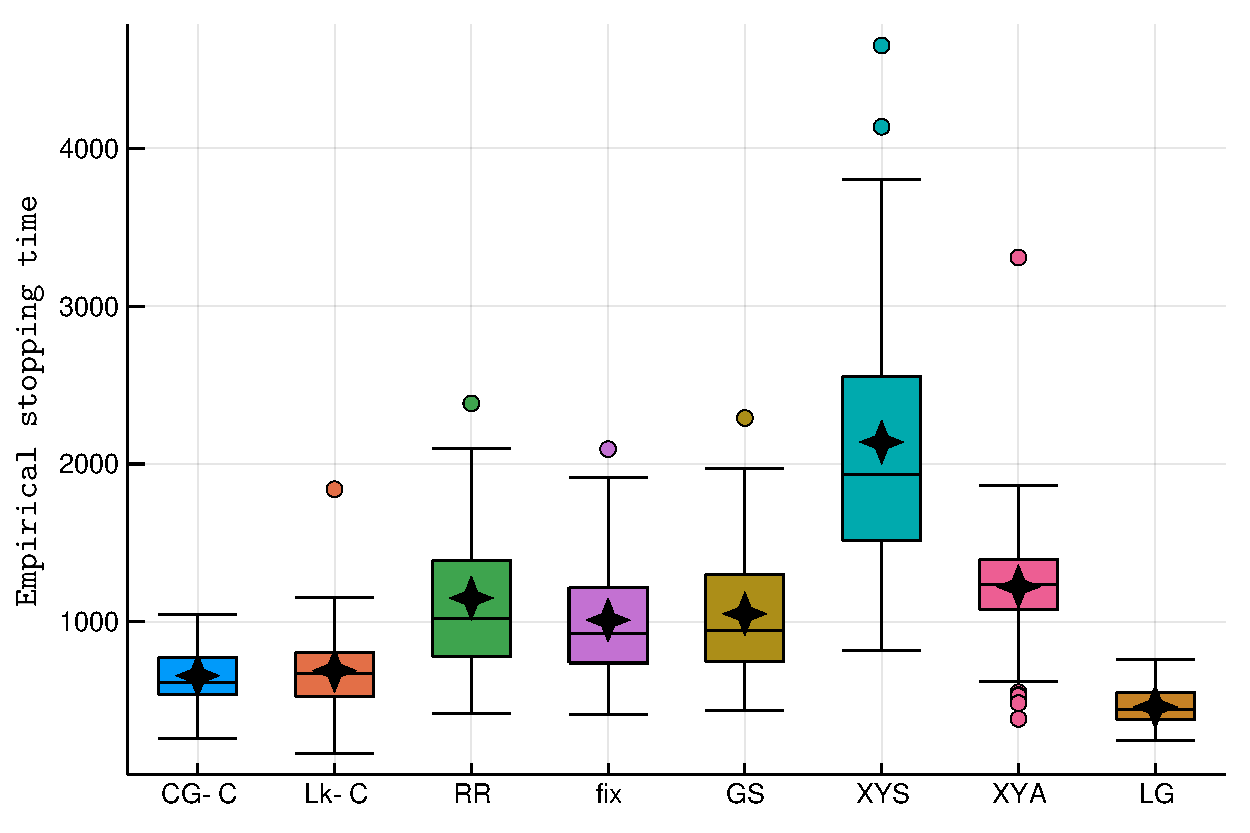
\includegraphics[clip, width= 0.33\textwidth]{Chapter4/img/bai_dim_10}
 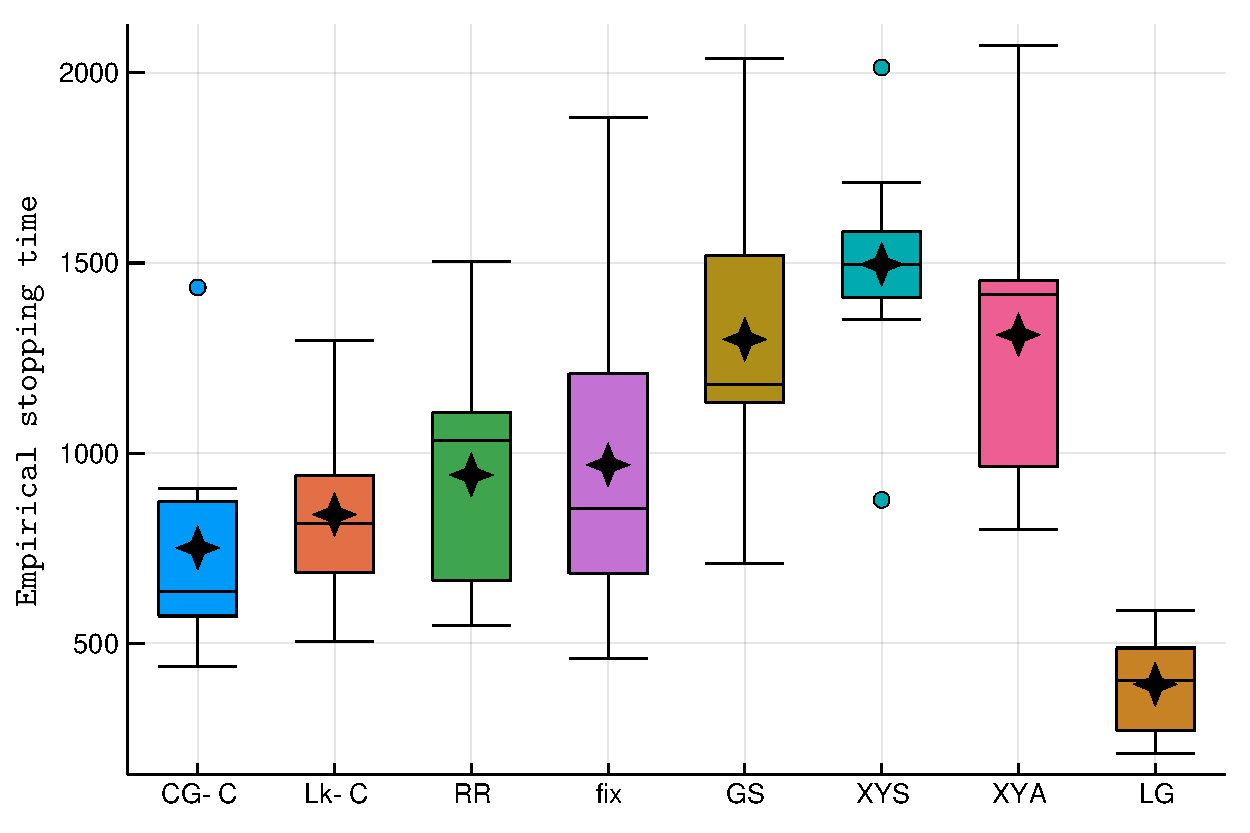
\includegraphics[clip, width= 0.34\textwidth]{Chapter4/img/bai_dim_12}
 \caption{Sample complexity of different linear BAI sampling rules over random unit sphere vectors with $d=6, 8, 10, 12$ from left to right.}
 \label{fig:sample_complexity_2}
\end{figure}

We stress that although the main focus of this chapter is theoretical, with algorithms that are asymptotically optimal, our methods are also competitive with earlier algorithms experimentally.
